\subsection{Address Translation}
\label{sec:paging}

Modern OS kernels rely on address translation to manage the access of
applications to the memory address space (\S~\ref{sec:address_spaces}). This
mechanism lets the kernel multiplex DRAM among multiple application processes,
isolate the processes from each other, and restrict applications from accessing
memory-mapped devices directly. The latter two are necessary to prevent an
application's bugs from impacting other applications, or the OS kernel itself.
Hypervisors also use address translation to split up the DRAM among
operating systems that run concurrently, and to virtualize memory-mapped
devices.

The software running inside a SGX enclave is subject to address
translation, and the implementation of SGX relies heavily on the translation
implementation in Intel processors. This section summarizes the Intel-specific
software-visible details needed to understand SGX, while \S~\ref{sec:tlbs}
covers some architectural specifics. \cite{jacob1998virtual} describes the
generic concepts and applications of address translation.

The Intel architecture specifies many address translation modes, used to run
legacy software dating back to 1990 natively. Most modes are not necessary for
understanding SGX, so we only cover the translation modes used in modern 64-bit
operating systems and 64-bit cloud environments.

% Canonical Addressing: SDM vol1 S 3.3.7.1
% IA-32e Paging: SDM S 4.5

64-bit desktop operating systems use the addressing mode called IA-32e by
Intel's documentation, which translates 48-bit \textit{virtual addresses} into
\textit{physical addresses} of at most 52 bits\footnote{The size of a physical
  address is CPU-dependent, and is 40 bits for recent desktop CPUs and 44 bits
for recent high-end server CPUs.}.  Figure~\ref{fig:os_paging} illustrates the
address translation process. The bottom 12 bits of a virtual address are not
changed by the translation. The top 36 bits are grouped into four 9-bit indexes
used to navigate a data structure called \textit{the page tables}. Despite its
name, the data structure closely resembles a perfectly balanced 512-ary search
tree where nodes have fixed keys.  Each node is an array of 512 8-byte entries
that contain the physical addresses of the next-level children as well as some
flags. The address of the root node is stored in the CR3 register. The arrays
in the last-level nodes contain the physical addresses that are the result of
the address translation.

\begin{figure}[hbtp]
  \center{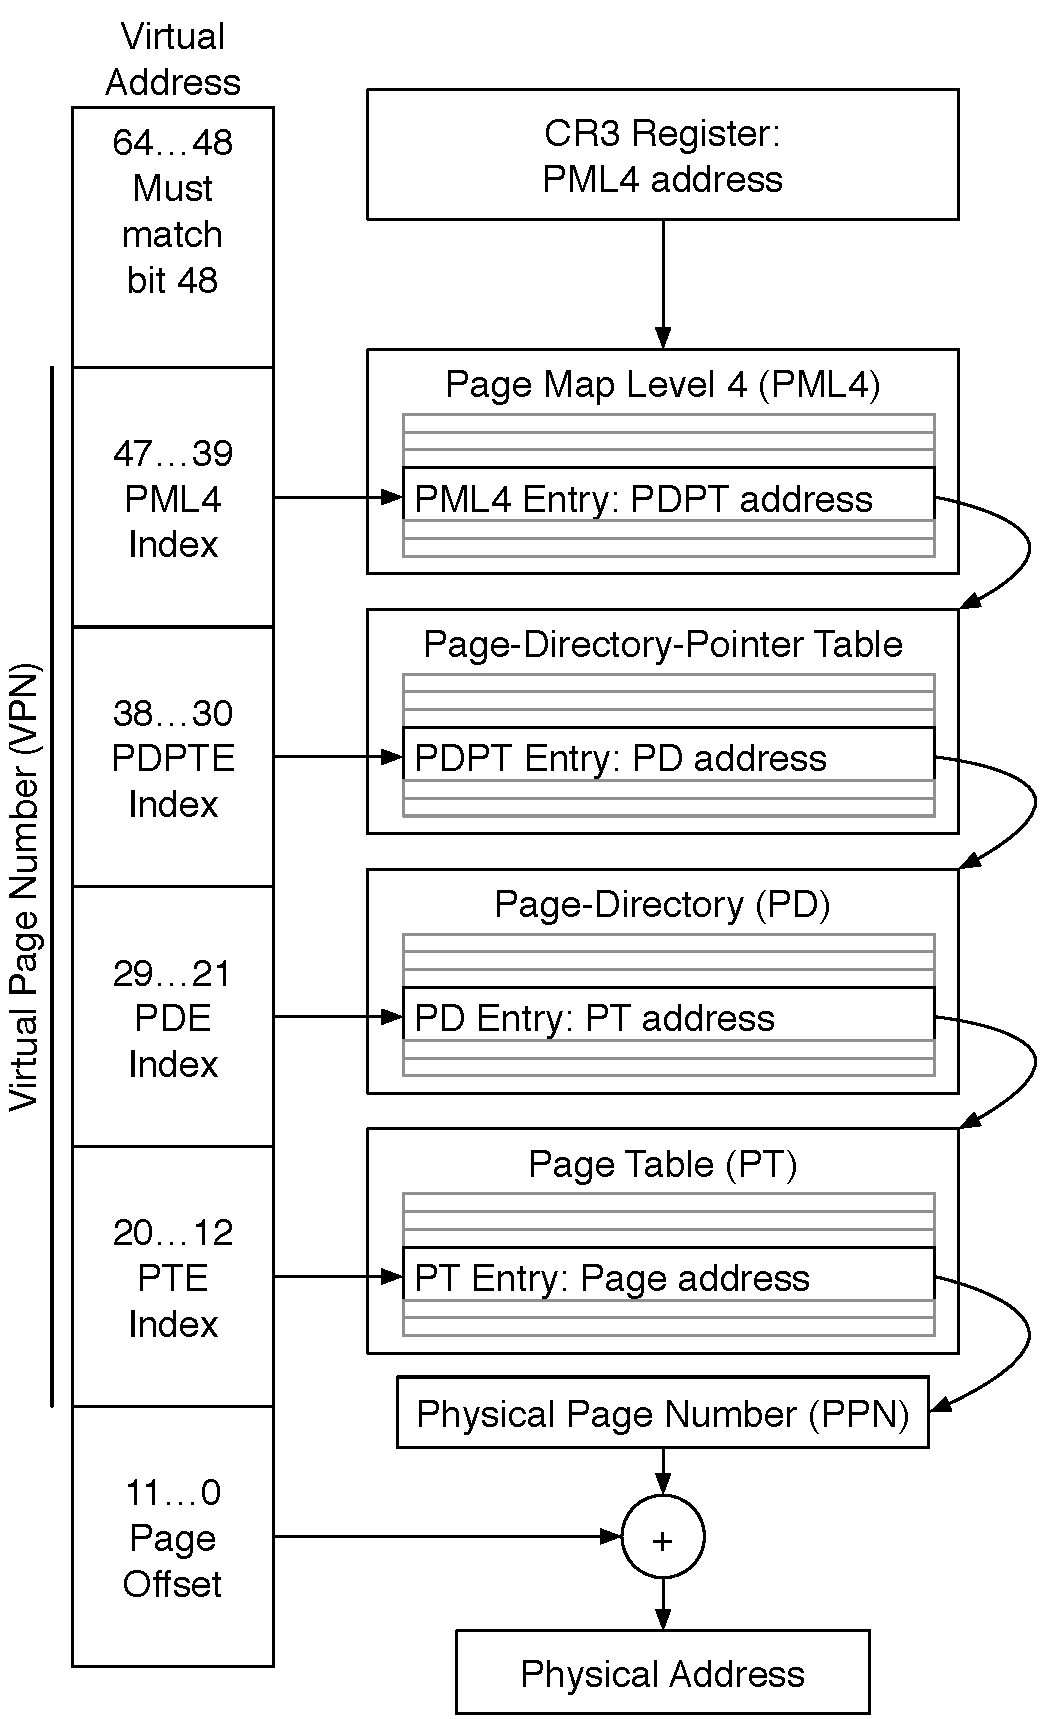
\includegraphics[width=85mm]{figures/os_paging.pdf}}
  \caption{
    IA-32e address translation takes in a 48-bit virtual address and outputs
    a 52-bit physical address.
  }
  \label{fig:os_paging}
\end{figure}

% VMX Support for Address Translation: SDM S 4.11

Hypervisors have access to another layer of address translation, named
\textit{extended page tables} (EPT), to multiplex the physical memory across
operating systems. When EPT are enabled, the process above is used to translate
from a virtual address into a \textit{guest-physical address}, effectively
giving each OS kernel the illusion that it controls the entire machine's RAM.
The translation from guest-physical addresses to actual physical addresses uses
the same process as above, except the physical address of the root node is
stored in the extended page table pointer (EPTP) field in the VM's control
structure (VMCS). Figure~\ref{fig:vmx_paging} illustrates the address
translation process in the presence of hardware virtualization.

\begin{figure}[hbtp]
  \center{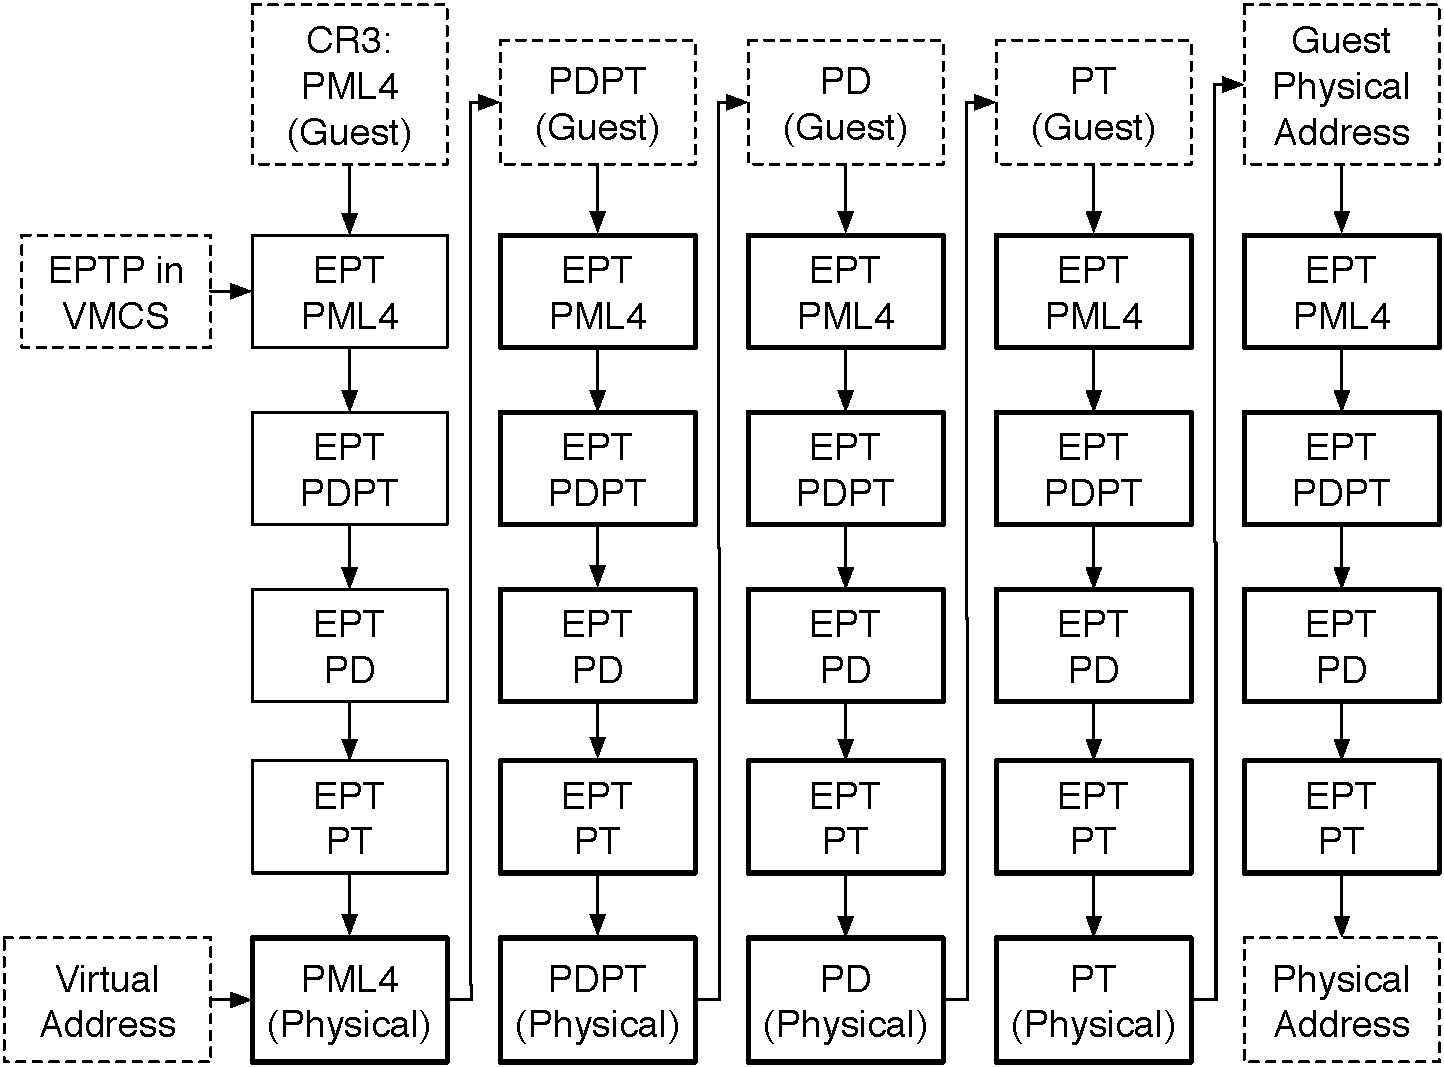
\includegraphics[width=85mm]{figures/vmx_paging.pdf}}
  \caption{
    Address translation when hardware virtualization is enabled. The
    kernel-managed page tables contain guest-physical addresses, so each level
    in the kernel's page table requires a full walk of the hypervisor's
    extended page table (EPT).  A translation requires up to 20 memory accesses
    (the bold boxes), assuming the physical address of the kernel's PML4 is
    cached.
  }
  \label{fig:vmx_paging}
\end{figure}

Each entry in the page tables has some boolean flags, in addition to the
pointer to the next level. The following flags are particularly interesting for
our goals. The \textit{present} (P) flag is set to 0 to indicate unused parts
of the address space, which do not have physical memory associated with them,
or pages that have been evicted from RAM to a cheaper and slower storage
medium.  The \textit{accessed} (A) flag is set to 1 by the CPU whenever the
address translation machinery reads a page table entry, and the \textit{dirty}
(D) flag is set to 1 by the CPU when an entry is accessed by a memory write
operation. The A and D flags give the hypervisor and kernel insight into
application memory access patterns, providing the input for the algorithms that
select which pages get to be evicted from RAM.

% Page-Level Protection: SDM S 5.11, S 5.11.{1,2,3,4}

Page table entries have flags that provide access control, in addition to the
flags supporting page swapping. The interesting flags are the \textit{writable}
(W) flag, which can be set to 0 to prohibit\footnote{Writes to non-writable
pages result in \#GP exceptions (\S~\ref{sec:faults}).} memory writes to a
page, the \textit{disable execution} (XD) flag, which can be set to 1 to
prevent instruction fetches from a page, and the \textit{supervisor} (S) flag,
which can be set to 1 to prohibit accesses from application software running at
ring 3.
